%\documentclass[letterpaper,draft]{beamer}
\documentclass[letterpaper,handout, mathserif]{beamer}
%\documentclass[letterpaper]{beamer}

%---multiple pages on one sheet, ADD for handout--
%\usepackage{pgfpages}
%\pgfpagesuselayout{4 on 1}[letterpaper, landscape, border shrink=1mm]
%-------------------------------------------------
\usepackage{amsmath,amsfonts}
%\usepackage{booktabs}
%\usepackage{mdwlist}
\usepackage{amsfonts}
%\usetheme{Copenhagen}
%\usetheme{warsaw}
\setbeamertemplate{navigation symbols}{}
\usepackage[english]{babel}
\def\ul{\underline}
% or whatever

\usepackage[latin1]{inputenc}
\subject{Talks}

\def\Sum{\sum\nolimits}
\def\Prod{\prod\nolimits}
\def\p{\mathrm P}
\def\E{\mathbb E}
\def\V{\mathrm Var}
\def\X{\mathcal{X}}
\def\typo#1{\alert{#1}}
%-------------Answers------------
\def\Hide#1#2{\ul{~~~\onslide<#1>{\alert{#2}}~~~}}
\def\hide#1#2{\ul{~~\onslide<#1>{\alert{#2}}~~}}
%------Centered Page Number------
\defbeamertemplate{footline}{centered page number}
{%
  \hspace*{\fill}%
  %\usebeamercolor[fg]{page number in head/foot}%
  %\usebeamerfont{page number in head/foot}%
  \small Lecture \chapnum\ - \insertframenumber%
  \hspace*{\fill}\vskip2pt%
}

%\usepackage{tikz}
%\usebackgroundtemplate{%
%\tikz\node[opacity=0.3] {\includegraphics[height=\paperheight,widht=\paperwidth]{ctanlion}};}

%\usebackgroundtemplate{%
%  %\rule{0pt}{\paperheight}%
%  \parbox[c][\paperheight][c]{\paperwidth}{\centering\includegraphics[width=.65\paperwidth]{UClogo.pdf}}
%  %\hspace*{\paperwidth}
%}

\def\chapnum{14}
%--------------------------------
\setbeamertemplate{footline}[centered page number]

\title{STAT253/317 Lecture \chapnum} \date{} \author{Cong Ma}
\begin{document}
% ----------------------------------------------------------------------
\begin{frame}\maketitle\begin{center}Chapter 7 \ Renewal Processes\end{center}\end{frame}
% ----------------------------------------------------------------------
\begin{frame}{Chapter 7 Renewal Processes}
Recall the interarrival times of a Poisson process are i.i.d exponential random variables.

\vfill 
A {\bf renewal process} is a counting process of which the interarrival times are i.i.d., but may not have an exponential distribution.\bigskip

\end{frame}
% ----------------------------------------------------------------------
\begin{frame}{Definition of a Renewal Process}
\begin{center}
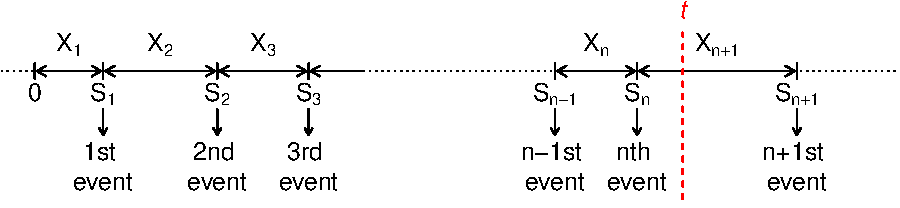
\includegraphics[width=\textwidth]{interarrivaltimes.pdf}
\end{center}
Let $X_1$, $X_2,\ldots$ be i.i.d random variables with $\E[X_i]<\infty,$ and $\p(X_i=0)  < 1$. Let
$$S_0=0, \quad S_n=X_1+\ldots+X_n, \;n\ge 1.$$
Define $$N(t)=\max\{n: S_n\le t\}.$$
Then $\{N(t), t\ge 0\}$ is called a \structure{\em renewal process}.
%where  are the interarrival times of events (a.k.a ``\structure{\em renewals},'') and $S_n$ is the time of the $n$th renewals.
\begin{itemize}
\item Events are called ``\structure{\em renewals}''. The interarrival times between events $X_1$, $X_2,\ldots$ are  also called ``renewals''
\item A more general definition allows the first renewal $X_1$ to be of a different distribution, called a \structure{\bf delayed renewal process}
\end{itemize}
\end{frame}
% ----------------------------------------------------------------------
\begin{frame}{Renewal Processes Are Well-Defined}
Renewal processes are well-defined in the sense that
 $$\p(\max\{n: S_n\le t\}<\infty)=1\quad\text{ for all }t>0.$$\pause
\begin{align*}
\text{By SLLN}&\Rightarrow\p\left(\lim_{n\to\infty}\frac{S_n}{n}=\E[X_1]\right)=1\\
&\Rightarrow\;\p\left(\lim_{n\to\infty}S_n =\infty\right)=1\\
&\Rightarrow\;\text{For any $t$, w/ prob. 1}\;S_n<t \quad\text{for only finitely many }n\\
&\Rightarrow\;\p(\max\{n: S_n\le t\}<\infty)=1\quad\text{for all }t>0
\end{align*}
\end{frame}
% ----------------------------------------------------------------------
\begin{frame}{Examples of Renewal Processes}
\begin{itemize}
\item Replacement of light bulbs: $N(t)=\#$ of replaced light bulbs by time $t$, is a renewal process
\item Consider a homogeneous, irreducible, positive recurrent, discrete time Markov chain, started from a state $i$.
Let
$$N_i(t)=\text{number of visits to state $i$ by time }t.$$
Then $\{N_i(t), t\ge 0\}$ is a renewal process.
\end{itemize}
\end{frame}
% ----------------------------------------------------------------------
\begin{frame}{Basic Properties of Renewal Processes}
\begin{itemize}[<+->]
\item $\p(\lim_{t\to\infty}N(t)=\infty)=1$\medskip

\underline{Reason}: $\lim_{t\to\infty}N(t)<\infty$ can happen only when $X_i=\infty$ for some $i$.
$$\left\{\lim_{t\to\infty}N(t)<\infty\right\}\subseteq \bigcup\nolimits_{i=1}^{\infty}\{X_i=\infty\}$$
However, as the interarrival times of a renewal process are required to have finite means
$\E[X_i]<\infty$, which implies $\p(X_i=\infty)=0$, we must have
$$\p\left(\lim_{t\to\infty}N(t)<\infty\right)
\le\p\left(\bigcup_{i=1}^{\infty}\{X_i=\infty\}\right)
\le\sum_{i=1}^{\infty}\p(X_i=\infty)=0.$$
\item Not memoryless in general\\[3pt]
$\Rightarrow$ No independent or stationary increments in general\\
$\p(N(t+h)-N(t)=1)$ depends on the current lifetime $A(t)=t-S_{N(t)}$
\end{itemize}
\end{frame}
% ----------------------------------------------------------------------
\begin{frame}{Things of Interest}
\begin{itemize}[<+->]
\item Distribution of $N(t)$: $$\p(N(t)=n),\quad n=0,1,2,\ldots$$
\item Renewal function: $$m(t)=\E[N(t)]$$
\item Residual life (a.k.a. excess life, overshoot, excess over the boundary):
$$B(t)=S_{N(t)+1}-t$$
\item Current age (a.k.a. current life, undershoot):
$$A(t)=t-S_{N(t)}$$
\item Total life: $C(t)=A(t)+B(t)$
\item Inspection paradox: $C(t)$ and the interarrival time $X_i$ have different distributions.
\end{itemize}
\end{frame}
% ----------------------------------------------------------------------
\begin{frame}{7.2. Distribution of $N(t)$}
Let $$F_n(t)=\p(S_n\le t)$$
be the CDF of the arrival time $S_n=X_1+\cdots+X_n$ of the $n$th event.
Observe that
\begin{eqnarray*}
%\text{$n$ events occur by time $t$}&\Leftrightarrow&\text{$n$th event occurs by time t}\\
\{N(t)\ge n\}&\Leftrightarrow& \{S_n\le t\}
\end{eqnarray*}
\begin{align*}
\text{Thus }\quad\quad\p(N(t) = n) &= \p(N(t) \ge n) - \p(N(t) \ge n+ 1)\\
&= \p(S_n \le t) - \p(S_{n+1} \le t)\\
&=F_{n}(t)-F_{n+1}(t)
\end{align*}
This formula looks simple but is generally \underline{USELESS} in practice since $F_{n}(t)$ is often intractable.
\end{frame}
% ----------------------------------------------------------------------
\begin{frame}{The Renewal Function $m(t)$}
Recall that if a random variable $X$ takes non-negative integer values $\{0,1,2,\ldots\}$, then
$\E[X]=\sum_{n=1}^{\infty}\p(X\ge n)$. Therefore the renewal function can be written as
\begin{align*}
m(t)=\E[N(t)]&=\sum_{n=1}^{\infty}\p(N(t)\ge n)\cr
&=\sum_{n=1}^{\infty}\p(S_n\le t)=\sum_{n=1}^{\infty}F_n(t)
\end{align*}

\vspace{-6pt}
\begin{itemize}
\item It can be shown that the renewal function $m(t)$ can uniquely determine the interarrival distribution $F$.
So the only renewal process with linear renewal function $m(t)=\lambda t$ is the Poisson process with rate $\lambda$.
\item The formula $m(t)=\sum_{n=1}^{\infty}F_n(t)$ is again generally \underline{useless} since $F_n(t)$ often times has no closed form expression.
We need more tools.
\end{itemize}
\end{frame}
% ----------------------------------------------------------------------
\begin{frame}{The Renewal Equation}
Conditioning on $X_1=x$, observe that
$$(N(t)|X_1=x)
=\begin{cases}
1+N(t-x) &\text{if }x\le t\\
0 & \text{if }x> t
\end{cases}
$$
Assuming that the interarrival distribution
$F$ is continuous with density function $f$. Then
\begin{align*}
m(t)&=\E[N(t)]=\int_0^{\infty}\E[N(t)|X_1=x]f(x)dx\\
&=\int_0^t(1+\E[N(t-x)])f(x)dx+\int_t^{\infty} 0 f(x)dx\\
&=\int_0^t(1+m(t-x))f(x)dx=F(t)+\int_0^t m(t-x)f(x)dx
\end{align*}
The equation $$m(t)=F(t)+\int_0^t m(t-x)f(x)dx$$ is called the \structure{\em renewal equation}.
%\textbf{Remark:} If $X_i$ do not have a continuous distribution, the general form of the renewal equation is
%$$m(t)=F(t)+\int_0^t m(t-x)dF(x).$$
\end{frame}
% ----------------------------------------------------------------------
\begin{frame}{Example 7.3}
Suppose the interarrival times $X_i$ are i.i.d. uniform on $(0, 1)$. The density and CDF of $X_i$'s are respectively
$$f(x)=
\begin{cases}
1 & \text{if }0\le x\le 1\\
0 & \text{otherwise}
\end{cases},\quad
F(x)=
\begin{cases}
0 & \text{if } x< 0\\[-3pt]
x & \text{if }0\le x\le 1\\[-3pt]
1 & \text{if } x> 1.
\end{cases}
$$
For $0\le t\le1$, the renewal equation is
$$m(t) = t +\int_0^{t} m(t-x)dx = t + \int_{0}^t m(x)dx$$
Differentiating the equation with respect to $t$ yields
$$m'(t)= 1+m(t)\Rightarrow \frac{d}{dt}(1+m(t))=1+m(t)\Rightarrow 1+m(t)=Ke^t.$$
or $m(t)=Ke^t-1$. Since $m(0)=0$, we can see that $K=1$ and obtain that
$m(t)=e^t-1$ for $0\le t\le1$.\par\medskip

What if $1\le t\le 2$?
\end{frame}
% ----------------------------------------------------------------------
\begin{frame}
For $1\le t\le 2$, $F(t)=1$, the renewal equation is
$$m(t) = 1 + \int_{0}^1 m(t-x)dx = 1 + \int_{t-1}^t m(x)dx$$
Differentiating the preceding equation yields
$$m'(t)= m(t)-m(t-1)=m(t)-[e^{t-1}-1]=m(t)+1-e^{t-1}$$
Multiplying both side by $e^{-t}$, we get
$$\underbrace{e^{-t}(m'(t)-m(t))}_{\frac{d}{dt}[e^{-t}m(t)]}=e^{-t}-e^{-1}$$
Integrating over $t$ from 1 to $t$, we get
\begin{align*}
e^{-t}m(t)&=e^{-1}m(1)+ e^{-1}\int_1^t e^{-(s-1)}-1ds\\
&=e^{-1}m(1)+e^{-1}[1-e^{-(t-1)}-(t-1)]\\
\Rightarrow m(t)&=e^{t-1}m(1)+e^{t-1}-1-e^{t-1}(t-1)\\
&=e^t+e^{t-1}-1-te^{t-1}\qquad (\text{Note }m(1)=e-1)
\end{align*}
\end{frame}
% ----------------------------------------------------------------------
\begin{frame}
In general for $n\le t\le n+1$, the renewal equation is
$$m(t) = 1 + \int_{t-1}^t m(x)dx\quad\Rightarrow\quad m'(t)= m(t)-m(t-1)$$
Multiplying both side by $e^{-t}$, we get
$$\frac{d}{dt}(e^{-t}m(t))=e^{-t}(m'(t)-m(t))=-e^{-t}m(t-1)$$
Integrating over $t$ from 1 to $t$, we get
$$e^{-t}m(t)=e^{-n}m(n)- \int_n^t e^{-s}m(s-1)ds$$
Thus we can find $m(t)$ iteratively.
\end{frame}
% ----------------------------------------------------------------------
\end{document}
\begin{frame}
\end{frame}
% ----------------------------------------------------------------------
